\subsection{Mann e Picard} \label{metodoMann}
O método proposto por Mann~e~Picard~\cite{mann} parte da problemática que, para ambientes com áreas bem iluminadas e outras pouco iluminadas, as câmeras convecionais acabam perdendo informações por não possuírem faixa dinâmica suficiente para representação de todos os valores de iluminação ali presentes. A solução de alguns fotógrafos para este problema é regular manualmente o tempo de exposição dos sensores da câmera, de forma que a perda seja a menor possível, ou valorizando apenas áreas de seu interesse. A solução proposta pelos autores restringe o problema à captura de várias imagens de uma mesma cena, variando apenas o tempo de exposição, sem que haja movimentação da câmera entre as capturas. Cada imagem possuirá informações relevantes de determinadas áreas da cena, e ao unir essas imagens obtem-se uma imagem com todas as informações de iluminação deste ambiente.
 
 
Para que se possa fazer a união das imagens é necessário saber o valor de iluminação que gerou o mapeamento para um dado pixel da imagem. Para isso, é necessário fazer o cálculo da inversa da função resposta da câmera, que é diferente para cada modelo de câmera no mercado, e muitas vezes é não-linear. Os autores propuseram um algoritmo para inferir a função resposta da câmera e assim calcular a inversa da mesma.

\subsubsection{Algoritmo para Inferir a Função Resposta} \label{metodoMannAlg}

Para o algoritmo são necessárias duas imagens $a$ e $b$ que foram capturadas em diferentes tempos de exposição, e estáticas uma em relação a outra. Considerando $k$ a razão do tempo de exposição de $b$ em relação ao de $a$ ($k > 1$), o objetivo é encontrar a função resposta $f$ da câmera que capturou as imagens seguindo os seguintes passos:

\begin{itemize}
\item É escolhido um pixel relativamente escuro na imagem $a$ posicionado em $(x_{0}, y_{0})$, denotado por $a(x_{0},y_{0})$. Sabe-se que um valor de irradiação de luz $q_{0}$ gerou o valor desse pixel a partir da aplicação da função resposta $f(q_{0}) = a(x_{0}, y_{0})$. 
\item Localiza-se o pixel na mesma posição na imagem $b$. Como as imagens são estáticas uma em relação a outra, sabe-se que $b(x_{0}, y_{0})$ possui o mesmo valor de irradiação de luz que $a(x_{0}, y_{0})$, porém com um tempo de exposição de $k$ vezes maior. Sendo assim volta-se à imagem $a$ e procura-se um pixel com o mesmo valor de $b(x_{0}, y_{0})$, denominado $a(x_{1}, y_{1}) = f(kq_{0})$.
\item Localiza o pixel $b(x_{1},y_{1})$ na imagem $b$, e procura-se na imagem $a$ um pixel com o valor $b(x_1,y_1)$ denominado $a(x_2, y_2) = f(k² q_0)$.
\item Ao aplicar a lógica do passo anterior sucessivamente para os pontos $(x_2, y_2), (x_3, y_3), ... , (x_n, y_n)$ é feito o mapeamento da não linearidade da função resposta.
\end{itemize}
Uma vez com os pontos encontrados elimina-se o termo $q_{0}$ por meio da mudança de escala, uma vez que não importa a unidade do eixo de irradiação \cite{mann}. O que leva nível de irradiação $q_{0}$ a ser considerado uma unidade de irradiação.

O método assume então que a função resposta possui a forma:
\begin{align} \label{eqMannTotal}
	f_{(q)} = \alpha + \beta q ^ \gamma
\end{align}
 Onde $\alpha$ pode ser considerado zero ao subtrair os valores dos pixels pelo valor obtido em uma imagem com tampa da lente colocada. O $\beta$ é um valor de escala e é arbitrário. E o $\gamma$ pode ser inferido atravez da equação:
	
\begin{align} \label{eqMannGama}
          b(x_{i},y_{i}) &= k^\gamma + a(x_{i},y_{i})
\end{align}


\subsubsection{Geração da Imagem HDR} \label{metodoMannGeracao}

O método proposto pelos autores para geração de uma imagem HDR se baseia na ideia que a derivada da função resposta da câmera em relação ao eixo logarítmico é proporcional à confiabilidade que o pixel apresenta. Sendo assim, para cada pixel da imagem, é feita uma média ponderada da confiabilidade que o pixel apresenta em cada tempo de exposição, possuindo maior peso aquele que possuir maior confiabilidade. Assim gerando um pixel HDR que foi formado a partir de informações de todas as exposições.

Seja um conjunto com $N$ imagens alinhadas entre si, variando apenas no tempo de exposição $t_{i}$, $i = 1 ... N$, onde cada imagem possui $M$ pixels representados por $I_{ij}$, $j = 1... M$, cada um com peso $p_{ij}$. A equação para inferir o valor de irradiação do pixel $x_{j}$ é dada por:

\begin{align} \label{eqMannGeracao}
          x_{j} = \frac{\sum\limits_{i \in N, j \in M}{p_{ij}\frac{f^{-1}(I_{ij})}{t_{i}}}}{\sum\limits_{i \in N, j \in M}{p_{ij}}}
\end{align}

\subsubsection{Resultados e Discussões} \label{metodoMannResultado}

O método em questão foi implementado na linguagem de programação C++, e foi utilizado um conjunto de imagens capturadas neste trabalho para a verificação dos resultados. Verificou-se que pelo fato do beta da equação \ref{eqMannTotal} ser arbitrário  a depender do valor atribuido ao mesmo pode-se haver uma incompatibilidade entre as funções respostas dos diferentes canais de cores da imagem, como mostrado na Figura \ref{figMannFigErr}.

\begin{figure}[H]
  \centering
  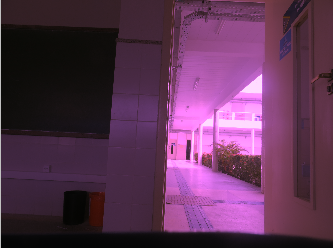
\includegraphics[height=6cm]{Mann/Ruin}
  \caption{Imagem HDR com diferença de escala entre os canais.}
  \label{figMannFigErr}
\end{figure}

Para solução deste problema foi utilizada a mesma solução proposta por Robertson \etal~\cite{robertson}, que estabelece que a função resposta deve sempre mapear o pixel com valor intermediário (128 para pixels com 8 bits) para o valor de uma unidade de luminosidade irradiada. Com essa modificação foi possível obter resultados satisfatórios na união dos canais HDR, conforme mostrado nas Figuras \ref{figMann1} e \ref{figMann2}.

\begin{figure}[H]
  \centering
  \subfloat[Imagem visualizada com baixo ganho.]
  {
    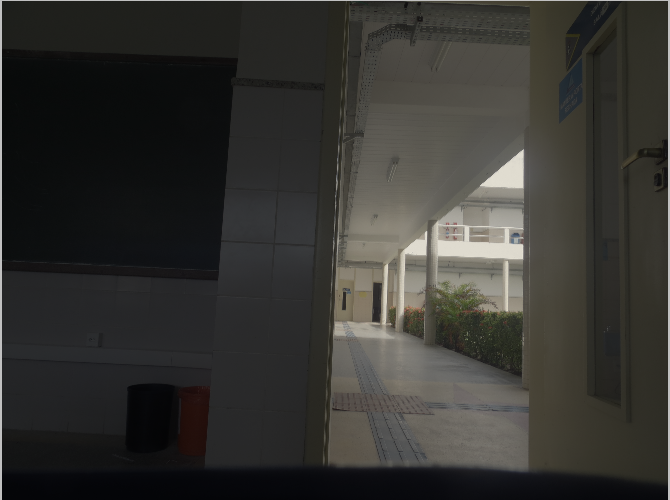
\includegraphics[height=6cm]{Mann/didaticaLow}
    \label{figMann1A}
  }
  \quad %espaco separador
  \subfloat[Imagem visualizada com alto ganho.]
  {
    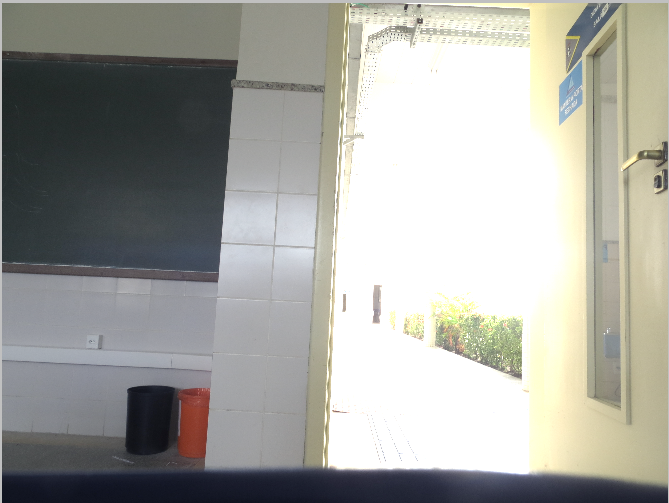
\includegraphics[height=6cm]{Mann/didaticaAlto}
    \label{figMann1B}
  }
  \caption{Imagem HDR obtida utilizando o método de Mann e Picard.}
  \label{figMann1}
\end{figure}

\begin{figure}[H]
  \centering
  \subfloat[Imagem visualizada com baixo ganho.]
  {
    
\includegraphics[height=6cm]{Mann/porquinhoLow}
    \label{figMann2A}
  }
  \quad %espaco separador
  \subfloat[Imagem visualizada com médio ganho.]
  {
    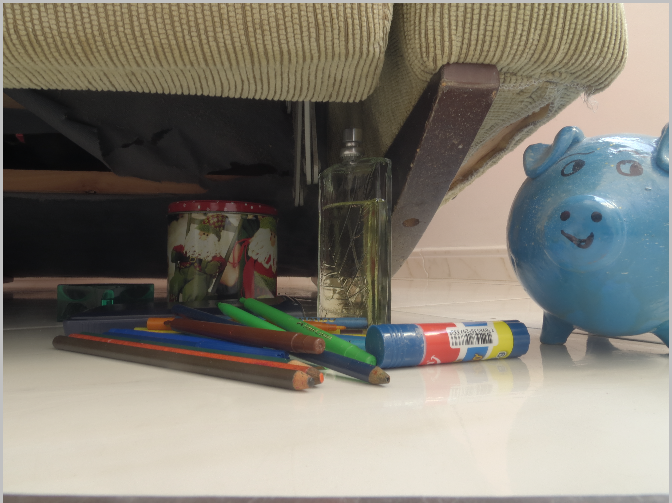
\includegraphics[height=6cm]{Mann/porquinhoMedio}
    \label{figMann2B}
  }
  \quad %espaco separador  
  \subfloat[Imagem visualizada com alto ganho.]
  {
    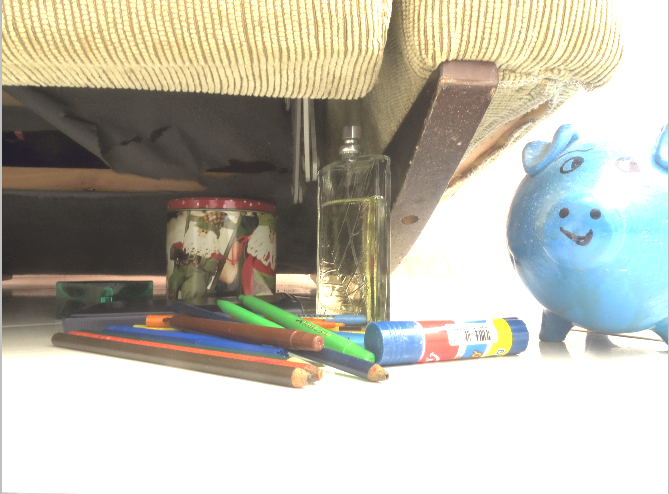
\includegraphics[height=6cm]{Mann/porquinhoAlto}
    \label{figMann2C}
  }
  \caption{Imagem HDR obtida utilizando o método de Mann e Picard.}
  \label{figMann2}
\end{figure}

A Figura \ref{figMannFR} mostra as funções resposta dos três canais obtidas utilizando o método proposto.

\begin{figure}[H]
  \centering
  \subfloat[Linear]
  {
    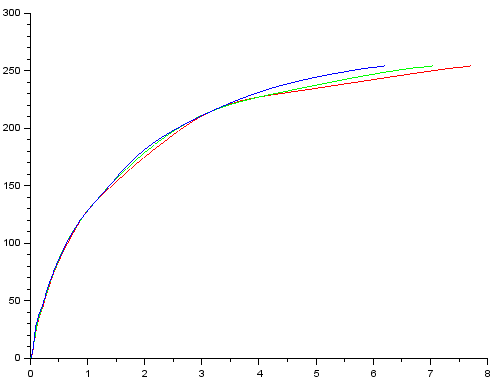
\includegraphics[height=6cm]{Mann/Fr-linear-total}
    \label{figMannFRA}
  }
  \quad %espaco separador
  \subfloat[Logaritmica]
  {
    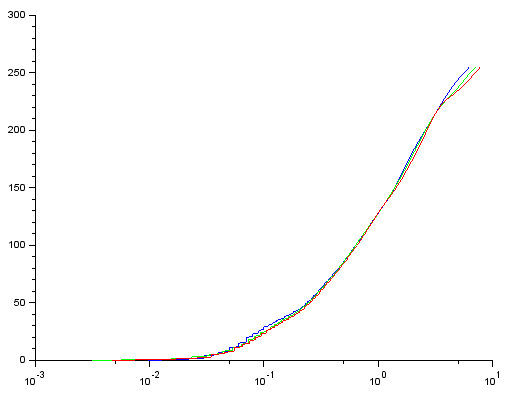
\includegraphics[height=6cm]{Mann/Fr-log-total}
    \label{figMannFRB}
  }
  \caption{Funções resposta da câmera no eixo linear (a) e no eixo logarítmico (b), referentes aos canais vermelho, verde e azul, obtidos com o método de Mann e Picard.}
  \label{figMannFR}
\end{figure}